\section{Propositional tableau}

In view of the impracticality of Hilbert-style proof systems, we introduce below an easier and more implementable method for determining a formula's validity --- \emph{tableaus}.

Here is a brief overview of how a tableau works. Suppose we want to check the satisfiability of a formula \(\phi\). This formula will be placed at the root of a binary tree, called a tableau. We use a variety of expansion rules to grow the tree until it is complete. An \emph{open} tableau indicates that \(\phi\) is satisfiable, while a \emph{closed} tableau indicates that \(\phi\) is unsatisfiable.

To determine the validity of a formula, simply construct a tableau for \(\neg\phi\). If the resultant tableau is open, then \(\neg\phi\) is satisfiable, so \(\phi\) is invalid. On the contrary, if the resultant tableau is closed, then \(\neg\phi\) must be unsatisfiable, so \(\phi\) is valid.


\subsection{Constructing a tableau}

In a tableau, every node is marked with a formula. To build a tableau for a formula \(\phi\), begin by placing \(\phi\) at the root of a binary tree. Then, we repeat the following process:
%
\begin{enumerate}
    \item Select a formula in the tree that has not been selected before. The formula must not be a literal.
    \item Choose the expansion rule (see below) that applies to the selected formula.
    \item For each leaf node, add new children nodes in accordance to the chosen expansion rule.
    \item Place a tick beside the selected formula to make sure we don't expand it again.
\end{enumerate}

There are two types of expansion rules:
%
\begin{itemize}
    \item \(\alpha\)-rules, which create one new child per leaf node; and
    \item \(\beta\)-rules, which create two new children per leaf node.
\end{itemize}

Figures \ref{fig:Ch03-alpha-rules} and \ref{fig:Ch03-beta-rules} depict the \(\alpha\)- and \(\beta\) rules respectively. Nodes that are newly created by each rule are highlighted in blue.


\begin{figure}[H]
    \centering
    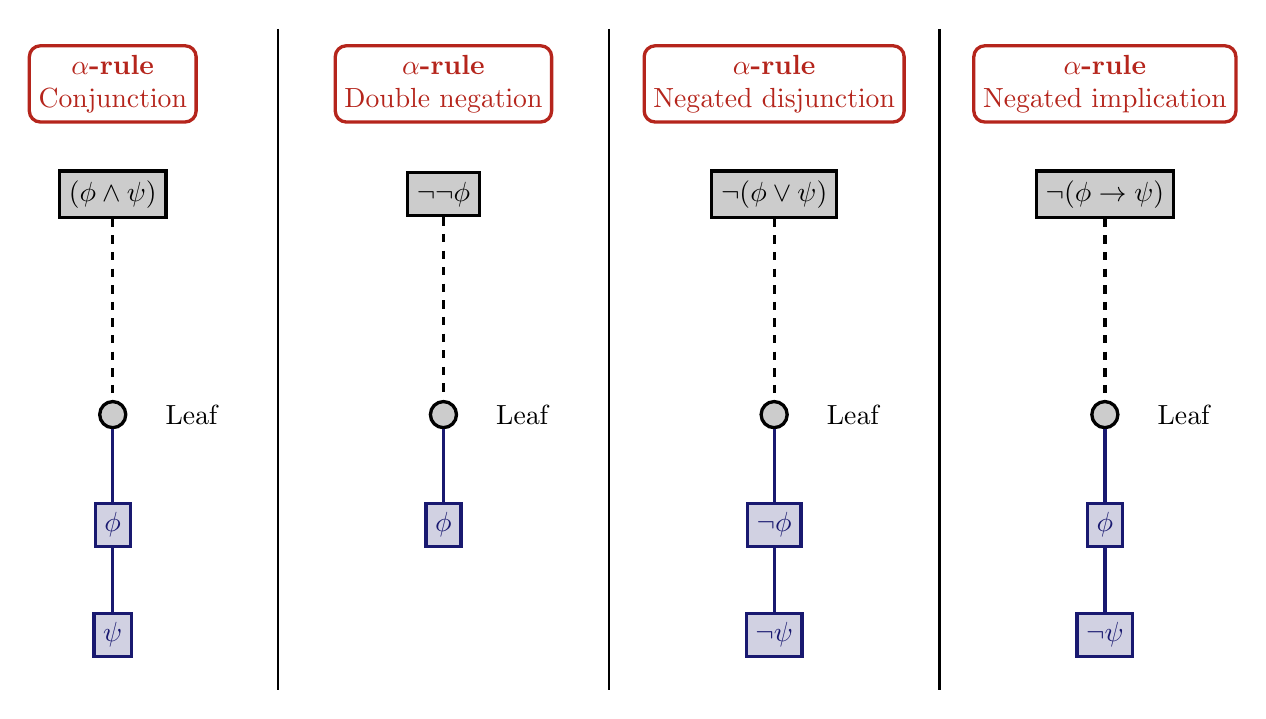
\begin{tikzpicture}[scale=1.4]
        \begin{scope}[shift={(0, 0)}]
            \node (root) at (0, 1)[draw=BrickRed, very thick, BrickRed, rounded corners, align=center] {\textbf{\(\alpha\)-rule} \\ Conjunction};

            \node (root) at (0, 0)[draw=black, very thick, fill=black!20] {\((\phi\land\psi)\)};

            \node (leaf) at (0, -2)[circle, draw=black, very thick, fill=black!20] {};

            \node [right of=leaf, black] {Leaf};

            \draw[dashed, very thick] (root) -- (leaf);

            \node (child1) at (0, -3)[draw=MidnightBlue, very thick, MidnightBlue, fill=MidnightBlue!20] {\(\phi\)};

            \node (child2) at (0, -4)[draw=MidnightBlue, very thick, MidnightBlue, fill=MidnightBlue!20] {\(\psi\)};

            \draw[very thick, MidnightBlue] (leaf) -- (child1) -- (child2);
        \end{scope}

        \begin{scope}[shift={(3, 0)}]
            \node (root) at (0, 1)[draw=BrickRed, very thick, BrickRed, rounded corners, align=center] {\textbf{\(\alpha\)-rule} \\ Double negation};

            \node (root) at (0, 0)[draw=black, very thick, fill=black!20] {\(\neg\neg\phi\)};

            \node (leaf) at (0, -2)[circle, draw=black, very thick, fill=black!20] {};

            \node [right of=leaf, black] {Leaf};

            \draw[dashed, very thick] (root) -- (leaf);

            \node (child1) at (0, -3)[draw=MidnightBlue, very thick, MidnightBlue, fill=MidnightBlue!20] {\(\phi\)};

            \draw[very thick, MidnightBlue] (leaf) -- (child1);
        \end{scope}

        \begin{scope}[shift={(6, 0)}]
            \node (root) at (0, 1)[draw=BrickRed, very thick, BrickRed, rounded corners, align=center] {\textbf{\(\alpha\)-rule} \\ Negated disjunction};

            \node (root) at (0, 0)[draw=black, very thick, fill=black!20] {\(\neg(\phi\lor\psi)\)};

            \node (leaf) at (0, -2)[circle, draw=black, very thick, fill=black!20] {};

            \node [right of=leaf, black] {Leaf};

            \draw[dashed, very thick] (root) -- (leaf);

            \node (child1) at (0, -3)[draw=MidnightBlue, very thick, MidnightBlue, fill=MidnightBlue!20] {\(\neg\phi\)};

            \node (child2) at (0, -4)[draw=MidnightBlue, very thick, MidnightBlue, fill=MidnightBlue!20] {\(\neg\psi\)};

            \draw[very thick, MidnightBlue] (leaf) -- (child1) -- (child2);
        \end{scope}

        \begin{scope}[shift={(9, 0)}]
            \node (root) at (0, 1)[draw=BrickRed, very thick, BrickRed, rounded corners, align=center] {\textbf{\(\alpha\)-rule} \\ Negated implication};

            \node (root) at (0, 0)[draw=black, very thick, fill=black!20] {\(\neg(\phi\rightarrow\psi)\)};

            \node (leaf) at (0, -2)[circle, draw=black, very thick, fill=black!20] {};

            \node [right of=leaf, black] {Leaf};

            \draw[dashed, very thick] (root) -- (leaf);

            \node (child1) at (0, -3)[draw=MidnightBlue, very thick, MidnightBlue, fill=MidnightBlue!20] {\(\phi\)};

            \node (child2) at (0, -4)[draw=MidnightBlue, very thick, MidnightBlue, fill=MidnightBlue!20] {\(\neg\psi\)};

            \draw[very thick, MidnightBlue] (leaf) -- (child1) -- (child2);
        \end{scope}
        
        \foreach \x in {1.5, 4.5, 7.5} {
            \draw[thick] (\x, 1.5) -- (\x, -4.5);
        }
    \end{tikzpicture}
    \caption{The four \(\alpha\)-rules for constructing propositional tableaus.}
    \label{fig:Ch03-alpha-rules}
\end{figure}


\begin{figure}[H]
    \centering
    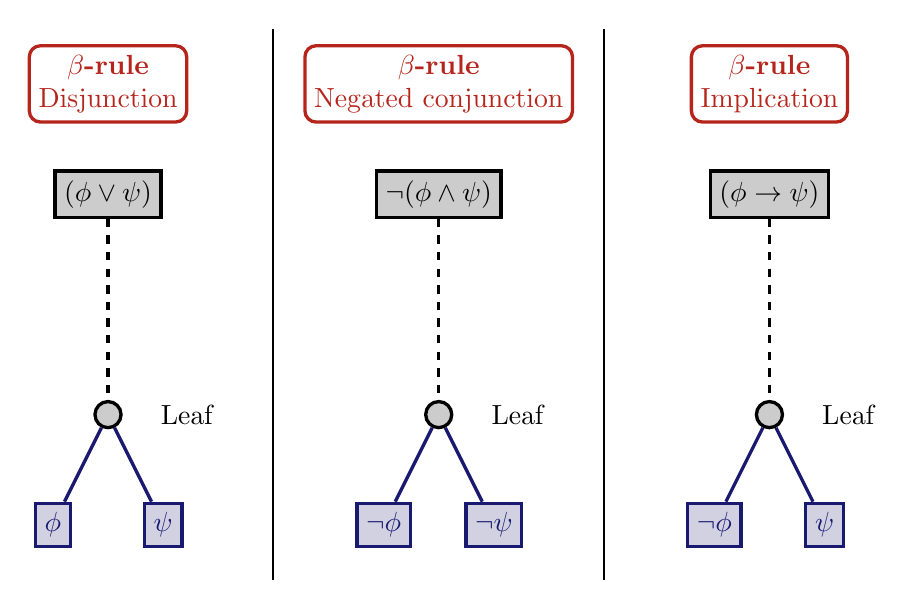
\begin{tikzpicture}[scale=1.4]
        \begin{scope}[shift={(0, 0)}]
            \node (root) at (0, 1)[draw=BrickRed, very thick, BrickRed, rounded corners, align=center] {\textbf{\(\beta\)-rule} \\ Disjunction};

            \node (root) at (0, 0)[draw=black, very thick, fill=black!20] {\((\phi\lor\psi)\)};

            \node (leaf) at (0, -2)[circle, draw=black, very thick, fill=black!20] {};

            \node [right of=leaf, black] {Leaf};

            \draw[dashed, very thick] (root) -- (leaf);

            \node (child1) at (-0.5, -3)[draw=MidnightBlue, very thick, MidnightBlue, fill=MidnightBlue!20] {\(\phi\)};

            \node (child2) at (0.5, -3)[draw=MidnightBlue, very thick, MidnightBlue, fill=MidnightBlue!20] {\(\psi\)};

            \draw[very thick, MidnightBlue] (leaf) -- (child1);
            \draw[very thick, MidnightBlue] (leaf) -- (child2);
        \end{scope}

        \begin{scope}[shift={(3, 0)}]
            \node (root) at (0, 1)[draw=BrickRed, very thick, BrickRed, rounded corners, align=center] {\textbf{\(\beta\)-rule} \\ Negated conjunction};

            \node (root) at (0, 0)[draw=black, very thick, fill=black!20] {\(\neg(\phi\land\psi)\)};

            \node (leaf) at (0, -2)[circle, draw=black, very thick, fill=black!20] {};

            \node [right of=leaf, black] {Leaf};

            \draw[dashed, very thick] (root) -- (leaf);

            \node (child1) at (-0.5, -3)[draw=MidnightBlue, very thick, MidnightBlue, fill=MidnightBlue!20] {\(\neg\phi\)};

            \node (child2) at (0.5, -3)[draw=MidnightBlue, very thick, MidnightBlue, fill=MidnightBlue!20] {\(\neg\psi\)};

            \draw[very thick, MidnightBlue] (leaf) -- (child1);
            \draw[very thick, MidnightBlue] (leaf) -- (child2);
        \end{scope}

        \begin{scope}[shift={(6, 0)}]
            \node (root) at (0, 1)[draw=BrickRed, very thick, BrickRed, rounded corners, align=center] {\textbf{\(\beta\)-rule} \\ Implication};

            \node (root) at (0, 0)[draw=black, very thick, fill=black!20] {\((\phi\rightarrow\psi)\)};

            \node (leaf) at (0, -2)[circle, draw=black, very thick, fill=black!20] {};

            \node [right of=leaf, black] {Leaf};

            \draw[dashed, very thick] (root) -- (leaf);

            \node (child1) at (-0.5, -3)[draw=MidnightBlue, very thick, MidnightBlue, fill=MidnightBlue!20] {\(\neg\phi\)};

            \node (child2) at (0.5, -3)[draw=MidnightBlue, very thick, MidnightBlue, fill=MidnightBlue!20] {\(\psi\)};

            \draw[very thick, MidnightBlue] (leaf) -- (child1);
            \draw[very thick, MidnightBlue] (leaf) -- (child2);
        \end{scope}
        
        \foreach \x in {1.5, 4.5} {
            \draw[thick] (\x, 1.5) -- (\x, -3.5);
        }
    \end{tikzpicture}
    \caption{The three \(\beta\)-rules for constructing propositional tableaus.}
    \label{fig:Ch03-beta-rules}
\end{figure}

In general, nodes located in the same branch\footnote{A \emph{branch} is defined as a path from the root of the tableau to one of its leaves.} are considered in conjunction while the different branches are considered to be disjuncted. As a result, a tableau is a tree-like representation of a formula that is a disjunction of conjunctions, à la disjunctive normal form (DNF).

A tableau is considered \emph{complete} if every node is either ticked (already expanded) or a literal. When a tableau is complete, we can determine the original formula's satisfiability as follows.
%
\begin{itemize}
    \item A branch containing both a propositional letter and its negation (\(p\) and \(\neg p\)) is said to be \emph{closed}, which we denote as \(\oplus\). Otherwise, it is \emph{open}.
    \item A tableau where all branches are closed is said to be \emph{closed}, meaning that the formula at its root is unsatisfiable. Contrarily, a tableau with at least one open branch is said to be \emph{open}, indicating that the formula is satisfiable.
\end{itemize}



\subsection{Example of constructing a tableau and converting to DNF}

To check if the formula
%
\[((p \lor q) \land (\neg p \rightarrow \neg q))\]
%
is satisfiable, we construct its tableau, as shown in figure \ref{fig:Ch03-satisfiability-tableau}.

Since only one of the four branches is closed, this formula is satisfiable. In fact, the literals in each open branch give a possible valuation that satisfies the given formula. For instance, the second branch from the left contains the literals \(p\) and \(\neg q\). This indicates that the formula is true when \(p\) is true and \(q\) is false.

\begin{figure}[H]
    \centering
    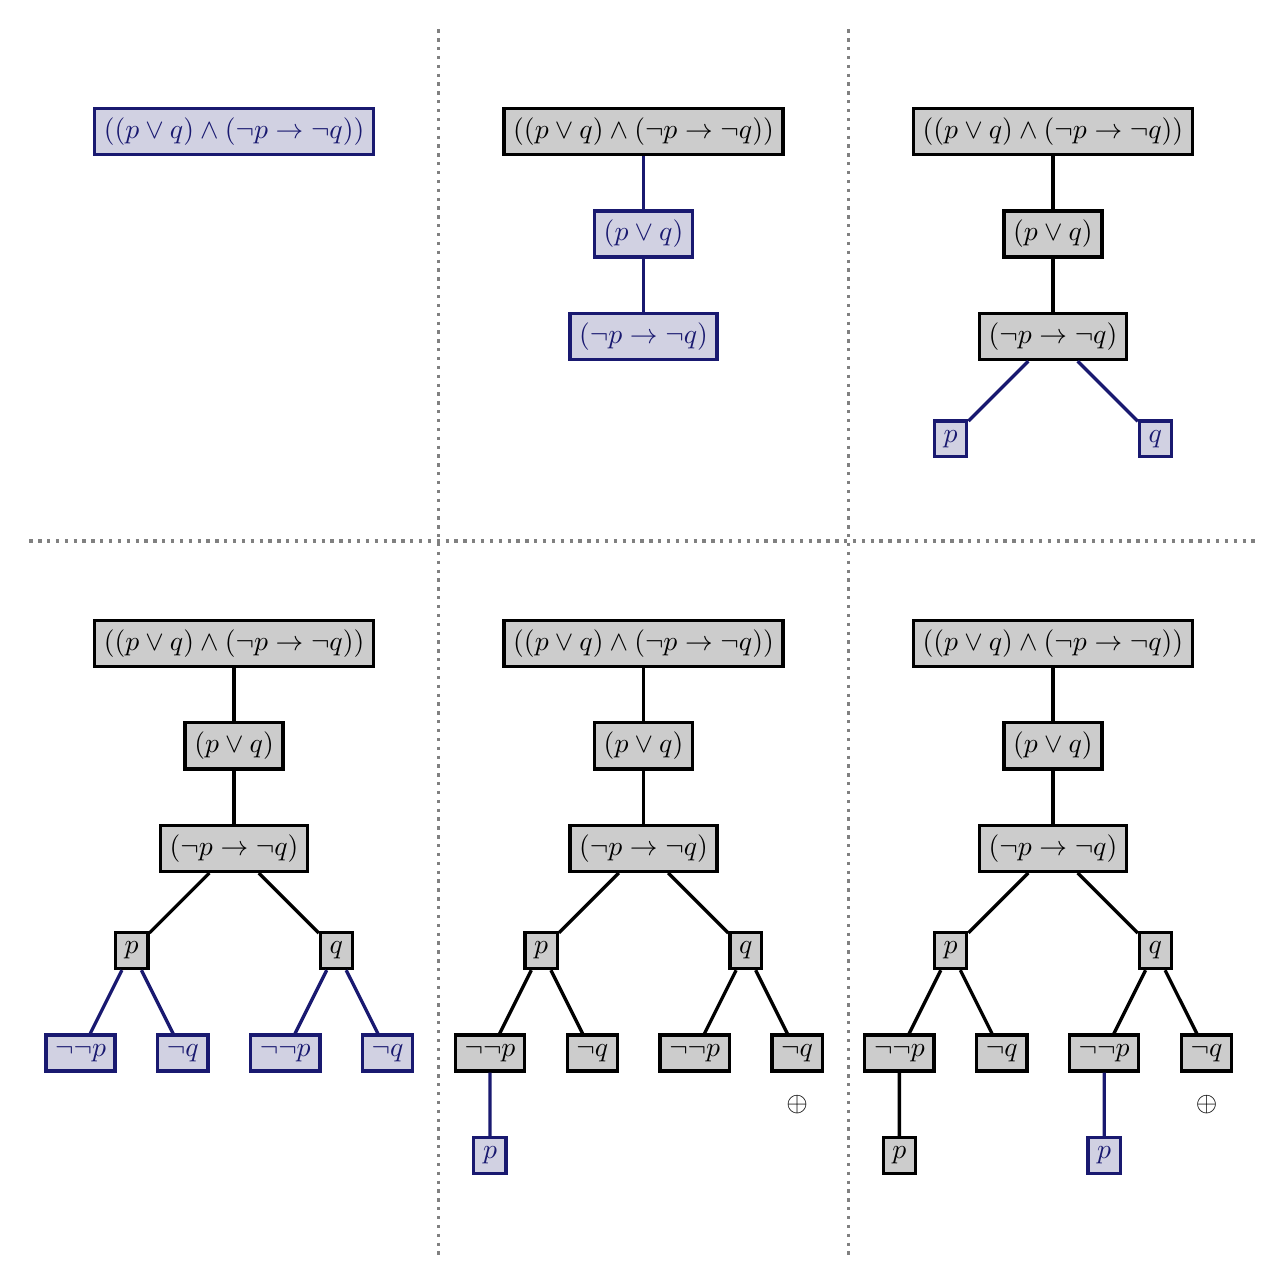
\begin{tikzpicture}[scale=1.3]
        \begin{scope}[shift={(0, 0)}]
            \node (0) at (0, 0)[draw=MidnightBlue, very thick, MidnightBlue, fill=MidnightBlue!20] {\(((p \lor q) \land (\neg p \rightarrow \neg q))\)};
        \end{scope}

        \begin{scope}[shift={(4, 0)}]
            \node (0) at (0, 0)[draw=black, very thick, fill=black!20] {\(((p \lor q) \land (\neg p \rightarrow \neg q))\)};
            \node[right of=0, xshift=30pt] {\checkmark};

            \node (1) at (0, -1)[draw=MidnightBlue, very thick, MidnightBlue, fill=MidnightBlue!20] {\((p \lor q)\)};

            \node (2) at (0, -2)[draw=MidnightBlue, very thick, MidnightBlue, fill=MidnightBlue!20] {\((\neg p \rightarrow \neg q)\)};

            \draw[MidnightBlue, very thick] (0) -- (1) -- (2);
        \end{scope}

        \begin{scope}[shift={(8, 0)}]
            \node (0) at (0, 0)[draw=black, very thick, fill=black!20] {\(((p \lor q) \land (\neg p \rightarrow \neg q))\)};
            \node[right of=0, xshift=30pt] {\checkmark};

            \node (1) at (0, -1)[draw=black, very thick, fill=black!20] {\((p \lor q)\)};
            \node[right of=1] {\checkmark};

            \node (2) at (0, -2)[draw=black, very thick, fill=black!20] {\((\neg p \rightarrow \neg q)\)};

            \node (3) at (-1, -3)[draw=MidnightBlue, very thick, MidnightBlue, fill=MidnightBlue!20] {\(p\)};

            \node (4) at (1, -3)[draw=MidnightBlue, very thick, MidnightBlue, fill=MidnightBlue!20] {\(q\)};

            \draw[black, very thick] (0) -- (1) -- (2);
            \draw[MidnightBlue, very thick] (2) -- (3);
            \draw[MidnightBlue, very thick] (2) -- (4);
        \end{scope}

        \begin{scope}[shift={(0, -5)}]
            \node (0) at (0, 0)[draw=black, very thick, fill=black!20] {\(((p \lor q) \land (\neg p \rightarrow \neg q))\)};
            \node[right of=0, xshift=30pt] {\checkmark};

            \node (1) at (0, -1)[draw=black, very thick, fill=black!20] {\((p \lor q)\)};
            \node[right of=1] {\checkmark};

            \node (2) at (0, -2)[draw=black, very thick, fill=black!20] {\((\neg p \rightarrow \neg q)\)};
            \node[right of=2, xshift=10pt] {\checkmark};

            \node (3) at (-1, -3)[draw=black, very thick, fill=black!20] {\(p\)};

            \node (4) at (1, -3)[draw=black, very thick, fill=black!20] {\(q\)};

            \node (5) at (-1.5, -4)[draw=MidnightBlue, very thick, MidnightBlue, fill=MidnightBlue!20] {\(\neg\neg p\)};

            \node (6) at (-0.5, -4)[draw=MidnightBlue, very thick, MidnightBlue, fill=MidnightBlue!20] {\(\neg q\)};

            \node (7) at (0.5, -4)[draw=MidnightBlue, very thick, MidnightBlue, fill=MidnightBlue!20] {\(\neg\neg p\)};

            \node (8) at (1.5, -4)[draw=MidnightBlue, very thick, MidnightBlue, fill=MidnightBlue!20] {\(\neg q\)};

            \draw[black, very thick] (0) -- (1) -- (2);
            \draw[black, very thick] (2) -- (3);
            \draw[black, very thick] (2) -- (4);
            \draw[MidnightBlue, very thick] (3) -- (5);
            \draw[MidnightBlue, very thick] (3) -- (6);
            \draw[MidnightBlue, very thick] (4) -- (7);
            \draw[MidnightBlue, very thick] (4) -- (8);
        \end{scope}

        \begin{scope}[shift={(4, -5)}]
            \node (0) at (0, 0)[draw=black, very thick, fill=black!20] {\(((p \lor q) \land (\neg p \rightarrow \neg q))\)};
            \node[right of=0, xshift=30pt] {\checkmark};

            \node (1) at (0, -1)[draw=black, very thick, fill=black!20] {\((p \lor q)\)};
            \node[right of=1] {\checkmark};

            \node (2) at (0, -2)[draw=black, very thick, fill=black!20] {\((\neg p \rightarrow \neg q)\)};
            \node[right of=2, xshift=10pt] {\checkmark};

            \node (3) at (-1, -3)[draw=black, very thick, fill=black!20] {\(p\)};

            \node (4) at (1, -3)[draw=black, very thick, fill=black!20] {\(q\)};

            \node (5) at (-1.5, -4)[draw=black, very thick, fill=black!20] {\(\neg\neg p\)};
            \node[above left of=5, xshift=15pt, yshift=-5pt] {\checkmark};

            \node (6) at (-0.5, -4)[draw=black, very thick, fill=black!20] {\(\neg q\)};

            \node (7) at (0.5, -4)[draw=black, very thick, fill=black!20] {\(\neg\neg p\)};

            \node (8) at (1.5, -4)[draw=black, very thick, fill=black!20] {\(\neg q\)};
            \node [below of=8, yshift=10pt] {\(\oplus\)};
            
            \node (9) at (-1.5, -5)[draw=MidnightBlue, very thick, MidnightBlue, fill=MidnightBlue!20] {\(p\)};

            \draw[black, very thick] (0) -- (1) -- (2);
            \draw[black, very thick] (2) -- (3);
            \draw[black, very thick] (2) -- (4);
            \draw[black, very thick] (3) -- (5);
            \draw[black, very thick] (3) -- (6);
            \draw[black, very thick] (4) -- (7);
            \draw[black, very thick] (4) -- (8);
            \draw[MidnightBlue, very thick] (5) -- (9);
        \end{scope}

        \begin{scope}[shift={(8, -5)}]
            \node (0) at (0, 0)[draw=black, very thick, fill=black!20] {\(((p \lor q) \land (\neg p \rightarrow \neg q))\)};
            \node[right of=0, xshift=30pt] {\checkmark};

            \node (1) at (0, -1)[draw=black, very thick, fill=black!20] {\((p \lor q)\)};
            \node[right of=1] {\checkmark};

            \node (2) at (0, -2)[draw=black, very thick, fill=black!20] {\((\neg p \rightarrow \neg q)\)};
            \node[right of=2, xshift=10pt] {\checkmark};

            \node (3) at (-1, -3)[draw=black, very thick, fill=black!20] {\(p\)};

            \node (4) at (1, -3)[draw=black, very thick, fill=black!20] {\(q\)};

            \node (5) at (-1.5, -4)[draw=black, very thick, fill=black!20] {\(\neg\neg p\)};
            \node[above left of=5, xshift=15pt, yshift=-5pt] {\checkmark};

            \node (6) at (-0.5, -4)[draw=black, very thick, fill=black!20] {\(\neg q\)};

            \node (7) at (0.5, -4)[draw=black, very thick, fill=black!20] {\(\neg\neg p\)};
            \node[above left of=7, xshift=15pt, yshift=-5pt] {\checkmark};

            \node (8) at (1.5, -4)[draw=black, very thick, fill=black!20] {\(\neg q\)};
            \node [below of=8, yshift=10pt] {\(\oplus\)};
            
            \node (9) at (-1.5, -5)[draw=black, very thick, fill=black!20] {\(p\)};

            \node (10) at (0.5, -5)[draw=MidnightBlue, very thick, MidnightBlue, fill=MidnightBlue!20] {\(p\)};

            \draw[black, very thick] (0) -- (1) -- (2);
            \draw[black, very thick] (2) -- (3);
            \draw[black, very thick] (2) -- (4);
            \draw[black, very thick] (3) -- (5);
            \draw[black, very thick] (3) -- (6);
            \draw[black, very thick] (4) -- (7);
            \draw[black, very thick] (4) -- (8);
            \draw[black, very thick] (5) -- (9);
            \draw[MidnightBlue, very thick] (7) -- (10);
        \end{scope}

        \draw[gray, very thick, dotted] (2, 1) -- (2, -11);
        \draw[gray, very thick, dotted] (6, 1) -- (6, -11);
        \draw[gray, very thick, dotted] (-2, -4) -- (10, -4);
    \end{tikzpicture}
    \caption{Constructing the tableau of \(((p \lor q) \land (\neg p \rightarrow \neg q))\). Read from left to right and from top to bottom.}
    \label{fig:Ch03-satisfiability-tableau}
\end{figure}

It follows that given the tableau of a formula, its DNF equivalent can be expressed as
%
\[
    \smashoperator{
        \mathop{
            \mathlarger{\mathlarger{\mathlarger{
                \lor
            }}}
        }
    }_{\text{open branch } \Theta}
    \left(
        \mathlarger{\mathlarger{\mathlarger{
            \land
        }}}
        \;\raisebox{2pt}{\(\{\text{literals in } \Theta\}\)}
    \right)
    \text{.}
\]

As always, the CNF of a formula can be obtained by negating the DNF form of its negation.